%(subject) (theme) (title)
\documentclass[11ptm]{jsarticle}

\usepackage{etoolbox}

\usepackage{array}

\usepackage{enumitem}

\usepackage{amsmath, newtxmath}

\usepackage[dvipdfmx]{graphicx}
%\usepackage[draft, dvipdfmx]{graphicx}

%\usepackage[hang, small, bf]{caption}
%\usepackage[subrefformat=parens]{subcaption}
%\captionsetup{compatibility=false}

\usepackage{listings, jlisting}

\lstset{
  basicstyle={\ttfamily\small},
  frame=tbrl,
  breaklines=true,
%  language=C,
  lineskip=-0.5ex,
  tabsize=2
}

\usepackage{ulinej}

\usepackage{tabularx}% 表(改変履歴)のため

\usepackage{hyperref}% ハイパーリンク付き参照
\usepackage{pxjahyper}% ハイパーリンク内の日本語の文字化け防止

\usepackage[margin=20mm]{geometry}% 余白調整用
% geometry settings
% geometry settings end

\renewcommand{\baselinestretch}{0.78}% 行間を少し狭める
\parindent = 0pt% 段落頭の字下げを無くす

\usepackage{fancybox}% fbox以外のboxコマンドを導入

\usepackage{lastpage}
\usepackage{fancyhdr}% ヘッダー・フッター装飾
% fancyhdr settings
\pagestyle{fancy}
\lhead{{\small\bf 一般ユーザ向けマニュアル}}
\chead{}
\rhead{{\small\bf \leftmark}}
\lfoot{}
\cfoot{\thepage}
\rfoot{}
% fansyhdr settings end

\usepackage{comment}% 複数行コメントアウト (comment環境)

\usepackage{caption}
\usepackage[subrefformat=parens]{subcaption}
\captionsetup[figure]{format=hang, font=small, name={\tt image}\ }

\makeatletter
\AtBeginDocument{
\let\c@figure\c@lstlisting
\let\thefigure\thelstlisting
\let\ftype@lstlisting\ftype@figure
}
\makeatother

\title{{\Huge POaM資産管理システム(仮称)\\操作マニュアル\\}一般ユーザ向け\\\Huge{第1版}}
\author{24 高橋祥吾\\26 田桑大輔\\29 田中稀尋\\30 谷川僚}
\date{}

%見出しの表示形式を再設定
\renewcommand{\thepart}{\arabic{part}}
\renewcommand{\thesection}{\ \arabic{section}章}
\renewcommand{\thesubsection}{\ \arabic{section}.\arabic{subsection}}

%%%%%%%%%%%%%%%%%%%
%%%%%%%%%%%%%%%%%%%
\begin{document}

%%%%%%%%%%
%タイトル
\setcounter{page}{0}

\maketitle
\thispagestyle{empty}

\clearpage

%%%%%%%%%%
%目次
\setcounter{page}{0}
\thispagestyle{empty}

\tableofcontents
\clearpage

\begin{comment}

%%%%%%%%%%
%\clearpage
\section{マニュアルとは}
\label{sec:マニュアルとは}
マニュアルには種類がある。
\begin{itemize}
  \item 操作マニュアル
  \item 業務マニュアル
  \item 障害対応マヌカハニー
  \item システムマニュアル
\end{itemize}\\
それぞれについて少し解説する。\\
操作マニュアルとは、システムの使い方、操作方法を記述するマニュアル。システムの起動や終了の仕方をはじめ、システムが備えるすべての機能の使い方、その機能を使う際の操作方法を詳細に記述。\\
業務マニュアルとは、システムを使った業務の進め方を記述するマニュアル。ひとつひとつの業務の流れ・手順を記述するとともに、流れ・手順のどの時点でシステムのどの機能を使うのかがわかるように記述する。機能の使い方や操作方法を記述する必要はない(操作マニュアルに任せる)。\\
障害対応マニュアルとは、システムに障害が生じたときの対応処理の方法を記述したもの。ただし、エンドユーザが自力で対応・解決できる範囲の障害だけに限る。要はQ$\&$A。\\
システムマニュアルとは、システムの仕組みや構造・全体的な構成などを基本からわかりやすく説明したもの。エンドユーザ向けであり、システム管理者やエンジニア向けのマニュアルのような詳細かつ専門的なものではなく、入門レベルの概要的なものになる。\\\\
我々が制作するのは授業的には操作マニュアルのみで十分だが、その他のマニュアルを制作してもソフトウェア工学の点数として評価される。また、障害対応マニュアルの一部を掲載すると丁寧。


%%%%%%%%%%
%\clearpage
\section{わかりやすい操作マニュアル制作のポイント}
\label{sec:わかりやすい操作マニュアル制作のポイント}
\url{https://www.science.co.jp/document_blog/26059/}

%%%%%
%\clearpage
\subsection{そもそも操作マニュアルとは}
\label{sec:そもそも操作マニュアルとは}
操作マニュアルとは文字通り、システムの操作方法を確認するためのドキュメント。マニュアルという立場上、操作マニュアルの多くは初心者や何も知らない顧客向けに作成される。よって、操作マニュアルの作成者は以下の点を意識する必要がある。
\begin{itemize}
  \item 初心者にも操作が理解しやすく記載されており、読後正しく操作ができる
  \item システムや機械を操作したあと、正しい操作だったかどうか、正解がわかる
  \item 困ったときに、すぐに該当のページに辿り着ける
\end{itemize}\\
世の中には、とりあえず操作手順を全部載せましたというマニュアルが存在している。分厚いだけのマニュアルは読み手の意欲を下げるので、ほとんど読まれることがない。また、直感的に操作できるシステムでは、作成しても操作マニュアルが読まれないケースがある。このような操作マニュアル未読のケースは、操作ミスや意図しない事故を発生させる可能性があり、大変危険である。\\
操作マニュアルの作成者は、先ほど挙げた3点を常に意識し、読了してもらえる操作マニュアルを完成しよう。

%%%%%
%\clearpage
\subsection{制作のポイント5つ}
\label{sec:制作のポイント5つ}
\begin{enumerate}
  \item 操作説明は網羅的に記載する
  \item 疑問点や注意事項は記載しておく
  \item 視覚的要素を用いる
  \item 操作の目的を記載する
  \item 操作の結果を記載する
\end{enumerate}
「Google検索からYahoo!のHPを開く」というケースで説明。

%%%%%
%\clearpage
\subsubsection{操作説明は網羅的に記載する}
\label{sec:操作説明は網羅的に記載する}
操作方法は細かいと良い。ただし冗長なものはわかりにくくなる。\\
操作内容の他にも、作業順、作業タイミング、操作者、条件などを記載するとよりわかりやすくなる。\\
\begin{lstlisting}
PC操作者 : Googleの検索バーに「yahoo」と打ち込み、Enterキー押下
検索結果が表示される
PC操作者 : 検索結果の一番上にある「Yahoo!JAPAN」をクリック
Yahoo!のHPを表示
\end{lstlisting}

%%%%%
%\clearpage
\subsubsection{疑問点や注意事項は記載しておく}
\label{sec:疑問点や注意事項は記載しておく}
操作にある程度慣れてくると疑問が湧くことがある。今回のケースで言えば、「Googleの検索履歴にYahoo!があるが、選択してもよいのか」など。このような疑問に対して、「入力履歴を選択しても問題ありません」などと記載しておくと、よりユーザビリティの高いマニュアルとなる。\\
また、注意事項や禁止操作も同時に記載すると良い。とはいえあらゆる疑問について記載していてはキリがないので、Q$\&$Aへ誘導するなどして、可読性とのバランスは取ったほうが良い。

%%%%%
%\clearpage
\subsubsection{視覚的要素を用いる}
\label{sec:視覚的要素を用いる}
文字だけでなく図や画像などを併せて操作マニュアルを記述しよう。

%%%%%
%\clearpage
\subsubsection{操作の目的を記載する}
\label{sec:操作の目的を記載する}
操作の目的を記載することで全体像の把握につながる。全体像の把握は作業効率の向上や作業重要性の理解につながる。\\
また、目次が目的ごとに並んでいれば、検索性が格段に上がる。自分のやりたい操作とページが瞬時に紐づくことで、作業が滞りなく進む。

%%%%%
%\clearpage
\subsubsection{操作の結果を記載する}
\label{sec:操作の結果を記載する}
今回のケースでいえば、以下のようなところ。
\begin{lstlisting}
  PC操作者 : Googleの検索バーに「yahoo」と打ち込み、Enterキー押下
  検索結果が表示される
\end{lstlisting}

\end{comment}

%%%%%%%%%%%%%%%%%%%%
%\clearpage
\part{前提}
\hrulefill


%%%%%%%%%%
%\clearpage
\section{はじめに}
\label{sec:はじめに}
POaM資産管理システム(以下、本システム)は、本校の資産を円滑かつ簡潔に管理するための、ブラウザ上で動作するオンラインWebアプリケーションです。\\
このPOaM資産管理システム操作マニュアル(以下、本マニュアル)は\ref{sec:動作環境}に則った環境を前提としています。システムを利用するためのURLにアクセスできない場合はネットワーク接続環境を確認してください。本マニュアルに掲載された画像は開発中のものです。\\
また、本マニュアルは通常権限を持ったユーザ向けです。


%%%%%%%%%%
%\clearpage
\section{動作環境}
\label{sec:動作環境}
本システムはIE9+のブラウザで動作します。\\
環境構築の方法は別紙\ 環境構築マニュアル\ をご参照ください。


%%%%%%%%%%%%%%%%%%%%
\clearpage
\part{操作説明}
\hrulefill


%%%%%%%%%%
%\clearpage
\section{起動・終了}
\label{sec:起動・終了}

%%%%%
%\clearpage
\subsection{システムの起動}
\label{sec:システムの起動}
ブラウザを開き、URLに接続します。接続に成功すると、{\tt image}\ \ref{fig:ログイン画面}が表示されます。\\
ログインについては\ref{sec:ログイン}を参照してください。

%%%%%
%\clearpage
\subsection{システムの終了}
\label{sec:システムの終了}
ブラウザのタブを閉じることでシステムを終了できます。\\
登録などの資産に関する作業をしているとき、\ovalbox{完了}ボタンを押す前にシステムを終了した場合、作業内容は保存されません。


%%%%%%%%%%
%\clearpage
\section{ログイン}
\label{sec:ログイン}
登録されたメールアドレスとパスワードをフォームに入力し、\ovalbox{1:ログイン}ボタンを押すことでログインできます。\\
ログインするとホーム画面({\tt image}\ \ref{fig:ホーム画面})が表示されます。\\
\ovalbox{2:非表示中}ボタンを押すと、入力中のパスワードの伏字を外すことができます。
\begin{figure}[h]
  \centering
  \begin{minipage}[h]{0.6\linewidth}
    \centering
    \fbox{
      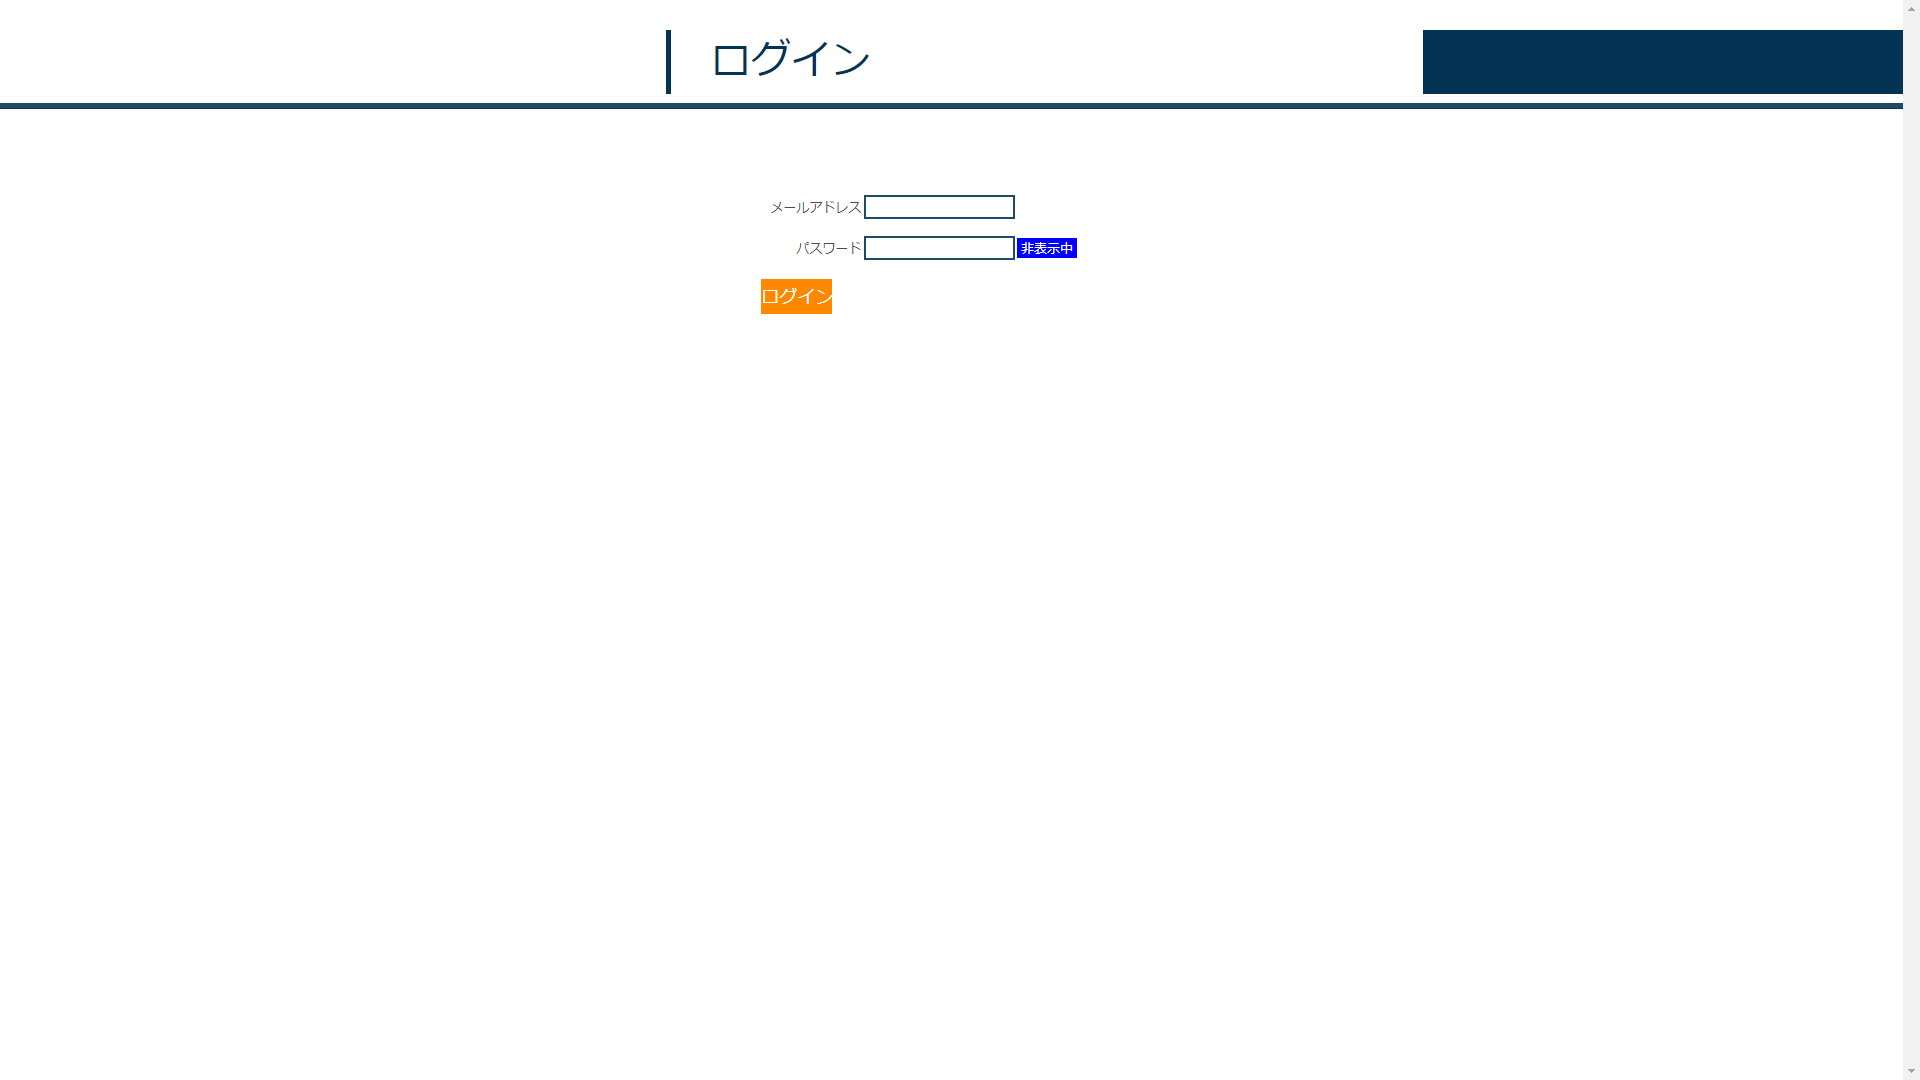
\includegraphics[keepaspectratio, width=\linewidth]{source/login.png}
    }
    \caption{\label{fig:ログイン画面}ログイン画面}
  \end{minipage}
  \hfill
  \begin{minipage}[h]{0.3\linewidth}
    \centering
    \fbox{
      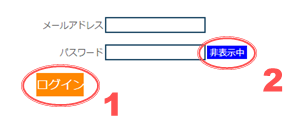
\includegraphics[keepaspectratio, width=\linewidth]{source/numered/login.png}
    }
    %\caption{\label{fig:}}
  \end{minipage}
\end{figure}\\


%%%%%%%%%%
\clearpage
\section{ホーム画面}
\label{sec:ホーム画面}
ホーム画面からは、本システムのほとんどの機能にアクセスできます。アクセスできる機能は以下の通りです。
\begin{itemize}
  \item 資産の登録 (\!\ref{sec:資産の登録})\qquad{\scriptsize \ovalbox{1:登録}}
  \item 資産の編集 (\!\ref{sec:資産の編集})\qquad{\scriptsize \ovalbox{2:編集}}
  \item プロフィールの編集 (\!\ref{sec:プロフィールの編集})\qquad{\scriptsize \ovalbox{4:ユーザ管理}}
  \item 資産情報の検索 (\!\ref{sec:資産の検索})\qquad{\scriptsize \ovalbox{5:検索機能}}
\end{itemize}
\begin{figure}[h]
  \centering
  \begin{minipage}[h]{0.6\linewidth}
    \centering
    \fbox{
      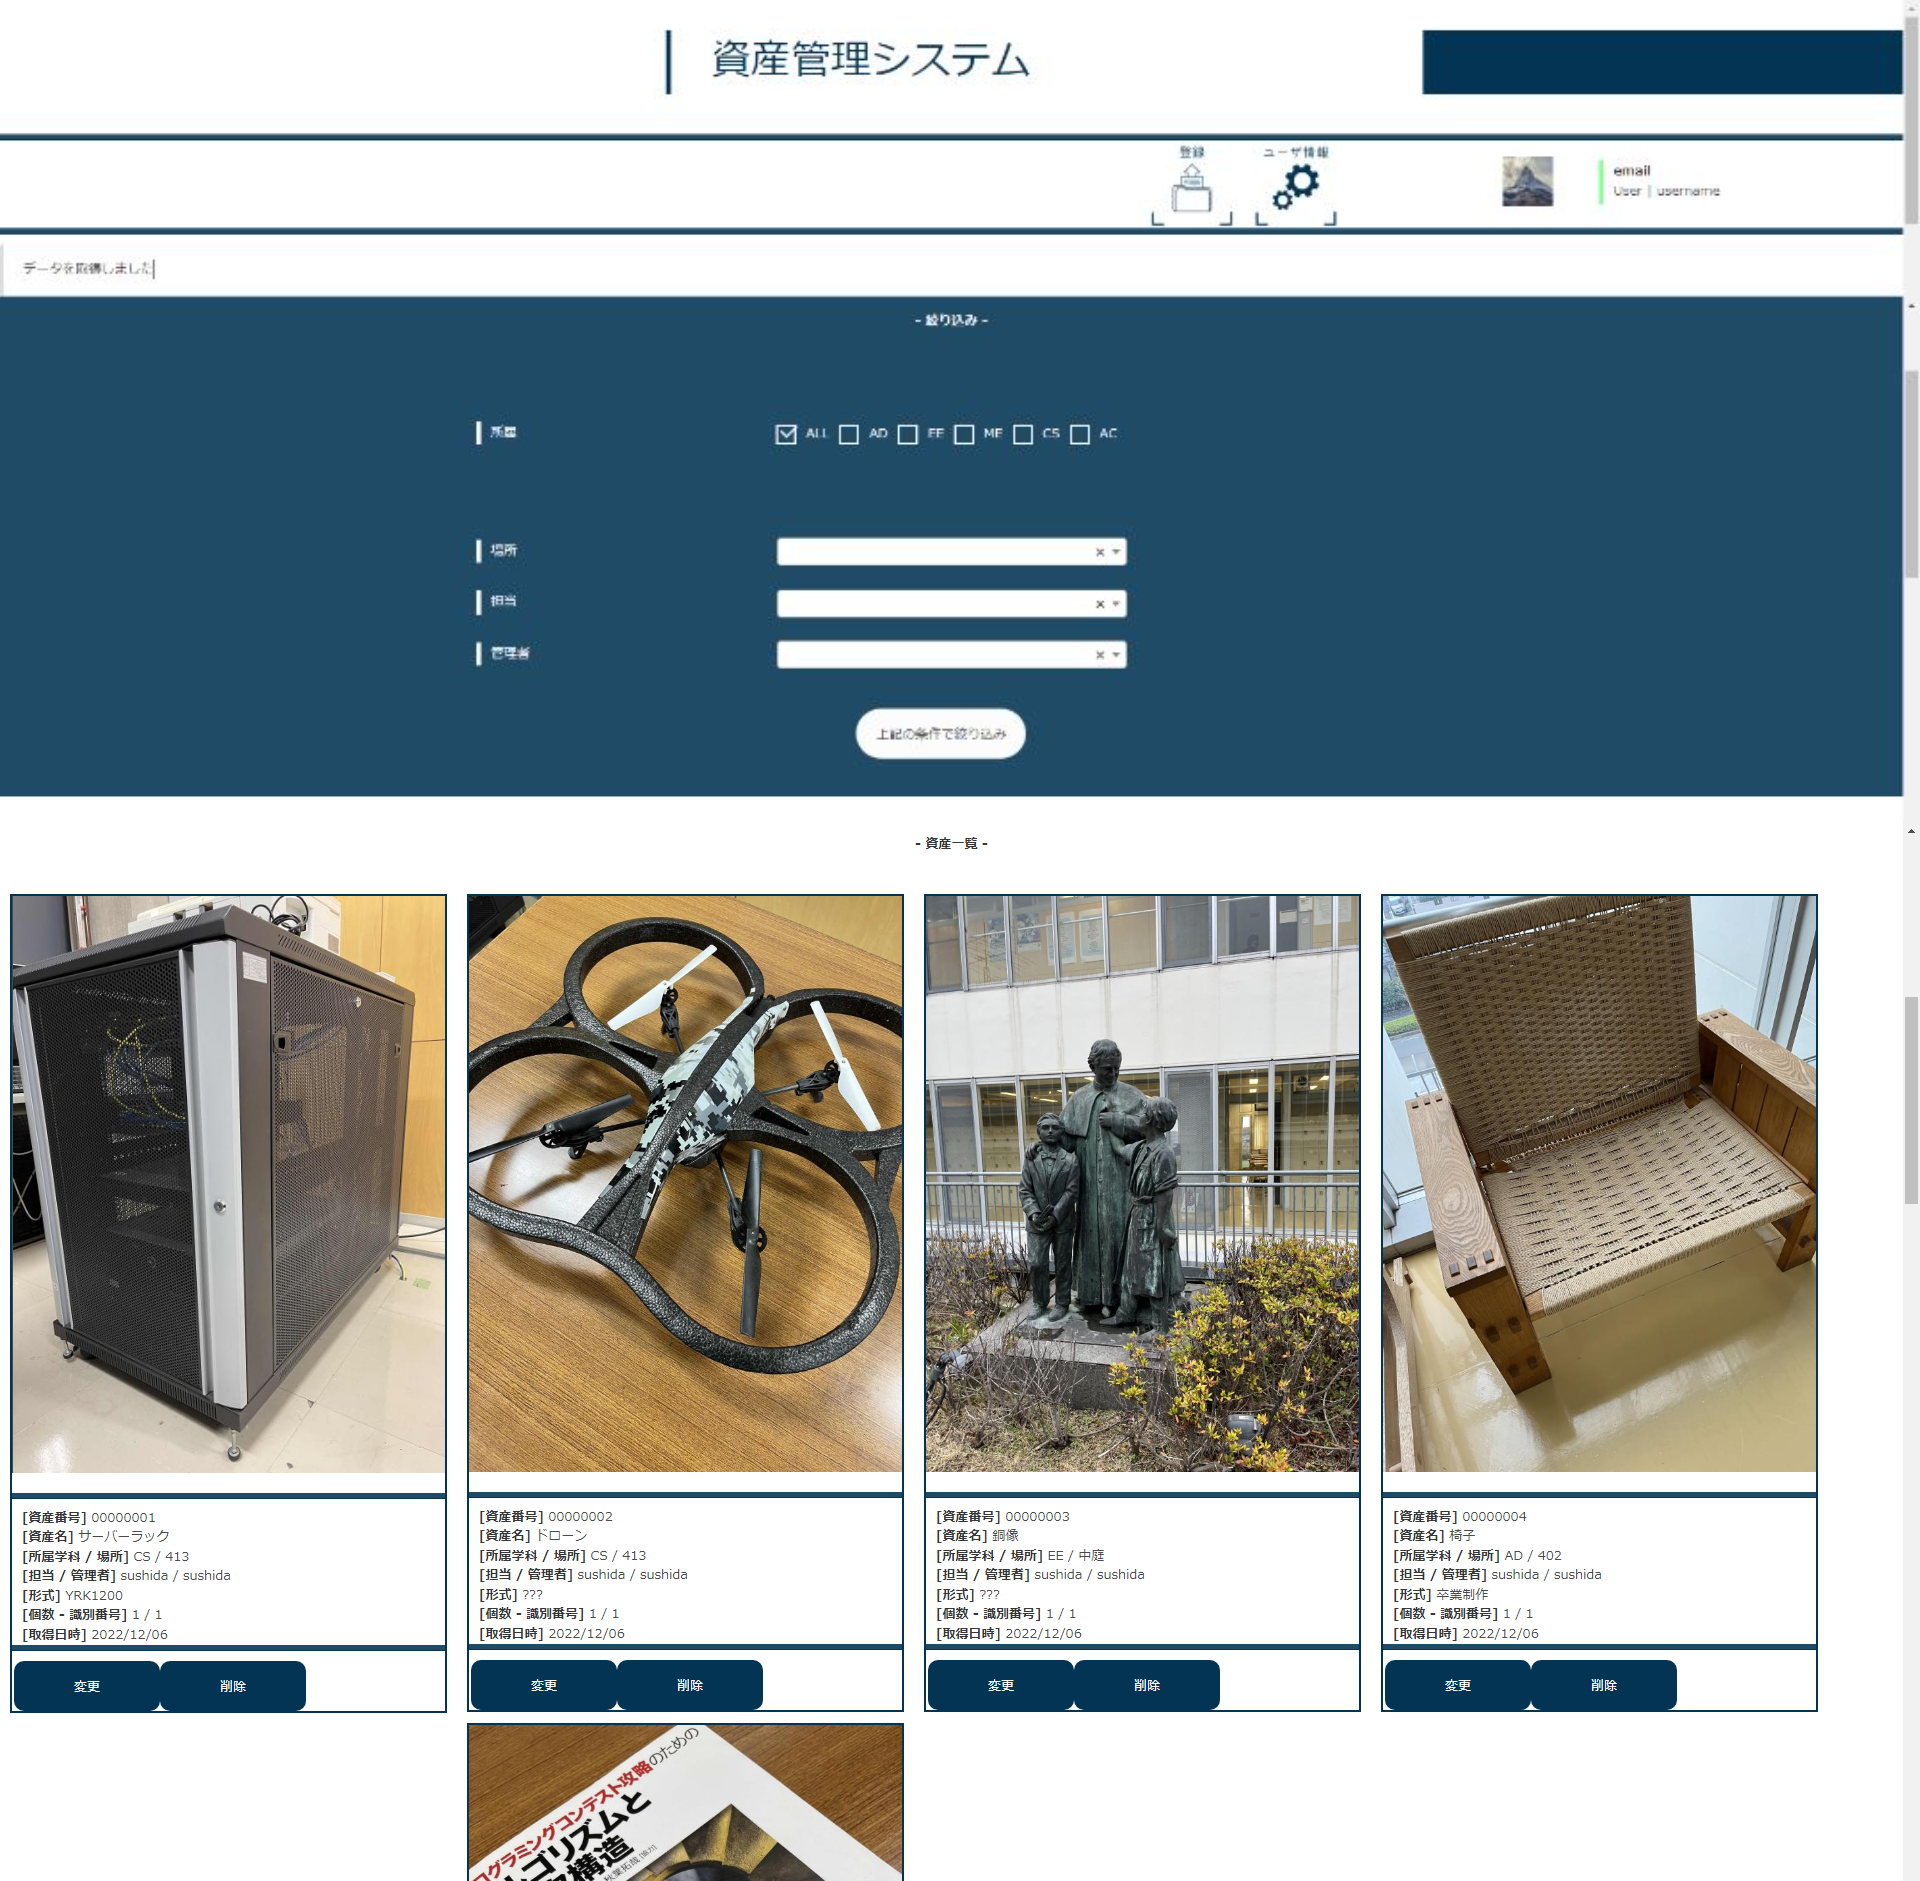
\includegraphics[keepaspectratio, width=\linewidth]{source/home.png}
    }
    \caption{\label{fig:ホーム画面}ホーム画面\\{\scriptsize スクロールした部分も含んでいます}}
  \end{minipage}
  \hfill
  \begin{minipage}[h]{0.3\linewidth}
    \centering
    \begin{minipage}[h]{\linewidth}
      \fbox{
        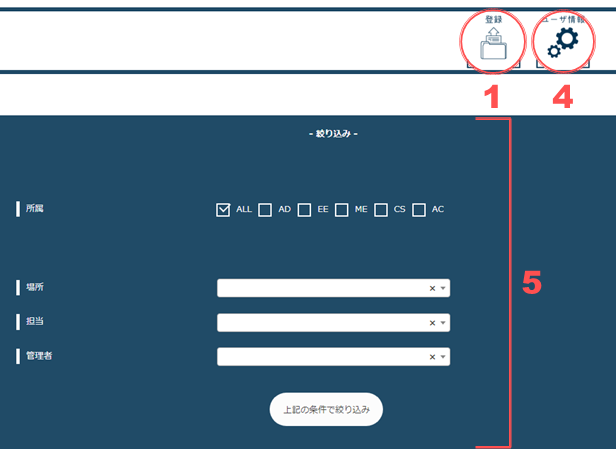
\includegraphics[keepaspectratio, width=\linewidth]{source/numered/home1.png}
      }
    \end{minipage}\\
    \bigskip
    \begin{minipage}[h]{\linewidth}
      \fbox{
        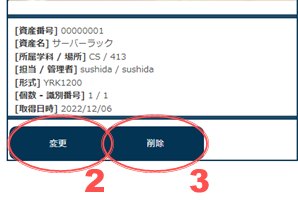
\includegraphics[keepaspectratio, width=\linewidth]{source/numered/home2.png}
      }
    \end{minipage}
  \end{minipage}
\end{figure}


%%%%%%%%%%
\clearpage
\section{資産の検索}
\label{sec:資産の検索}
ホーム画面({\tt image}\ \ref{fig:ホーム画面})の下部で資産の検索を行えます。\\
検索は項目別に絞り込んで行えます。絞り込み項目は所属、場所、担当、管理者となっており、これらを選択または入力して\ovalbox{上記の条件で絞り込み}ボタンを押すことで検索結果が変化します。
\begin{figure}[h]
  \centering
  \fbox{
    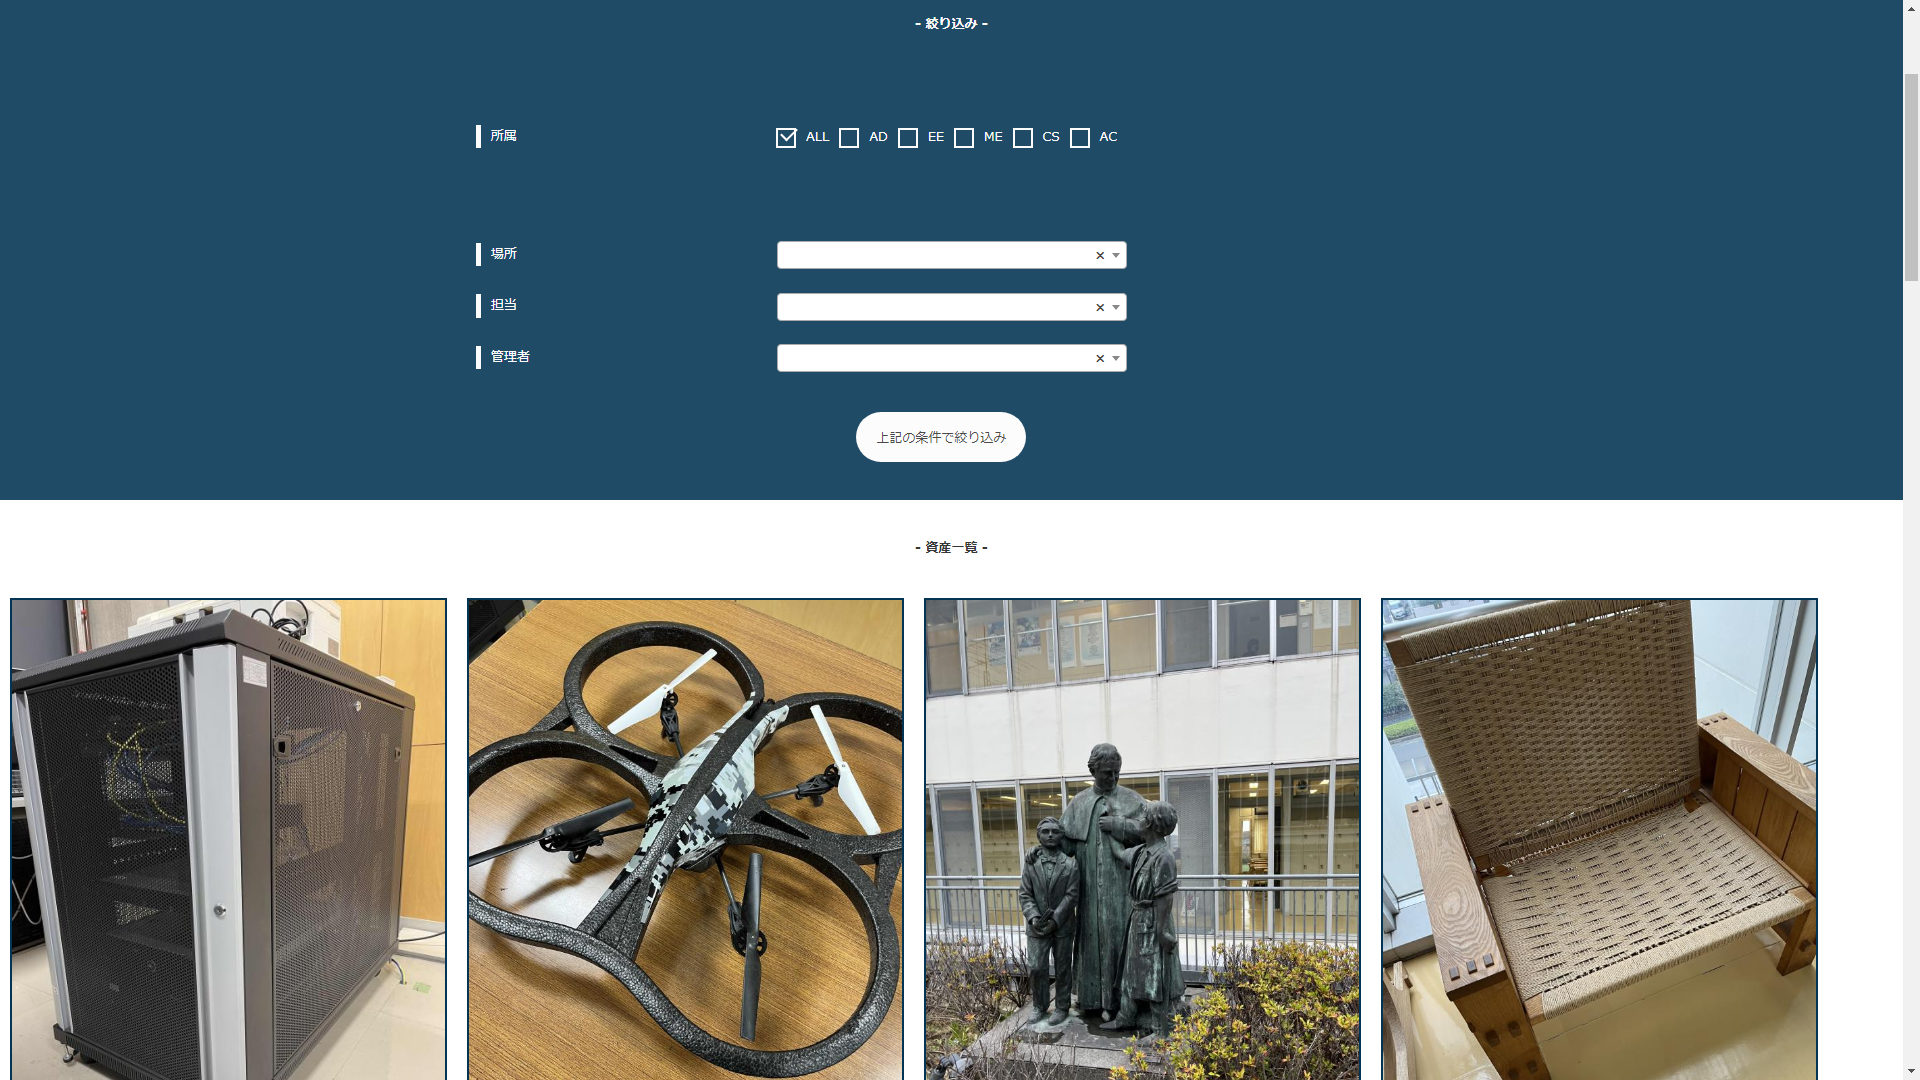
\includegraphics[keepaspectratio, width=0.8\linewidth]{source/search1.png}
  }
  \caption{\label{fig:検索}検索}
\end{figure}\\
たとえば、所属をADとEEにのみチェックを入れて\ovalbox{上記の条件で絞り込み}ボタンを押して検索すると{\tt image}\ \ref{fig:変化した検索画面}のようになります。
\begin{figure}[h]
  \centering
  \fbox{
    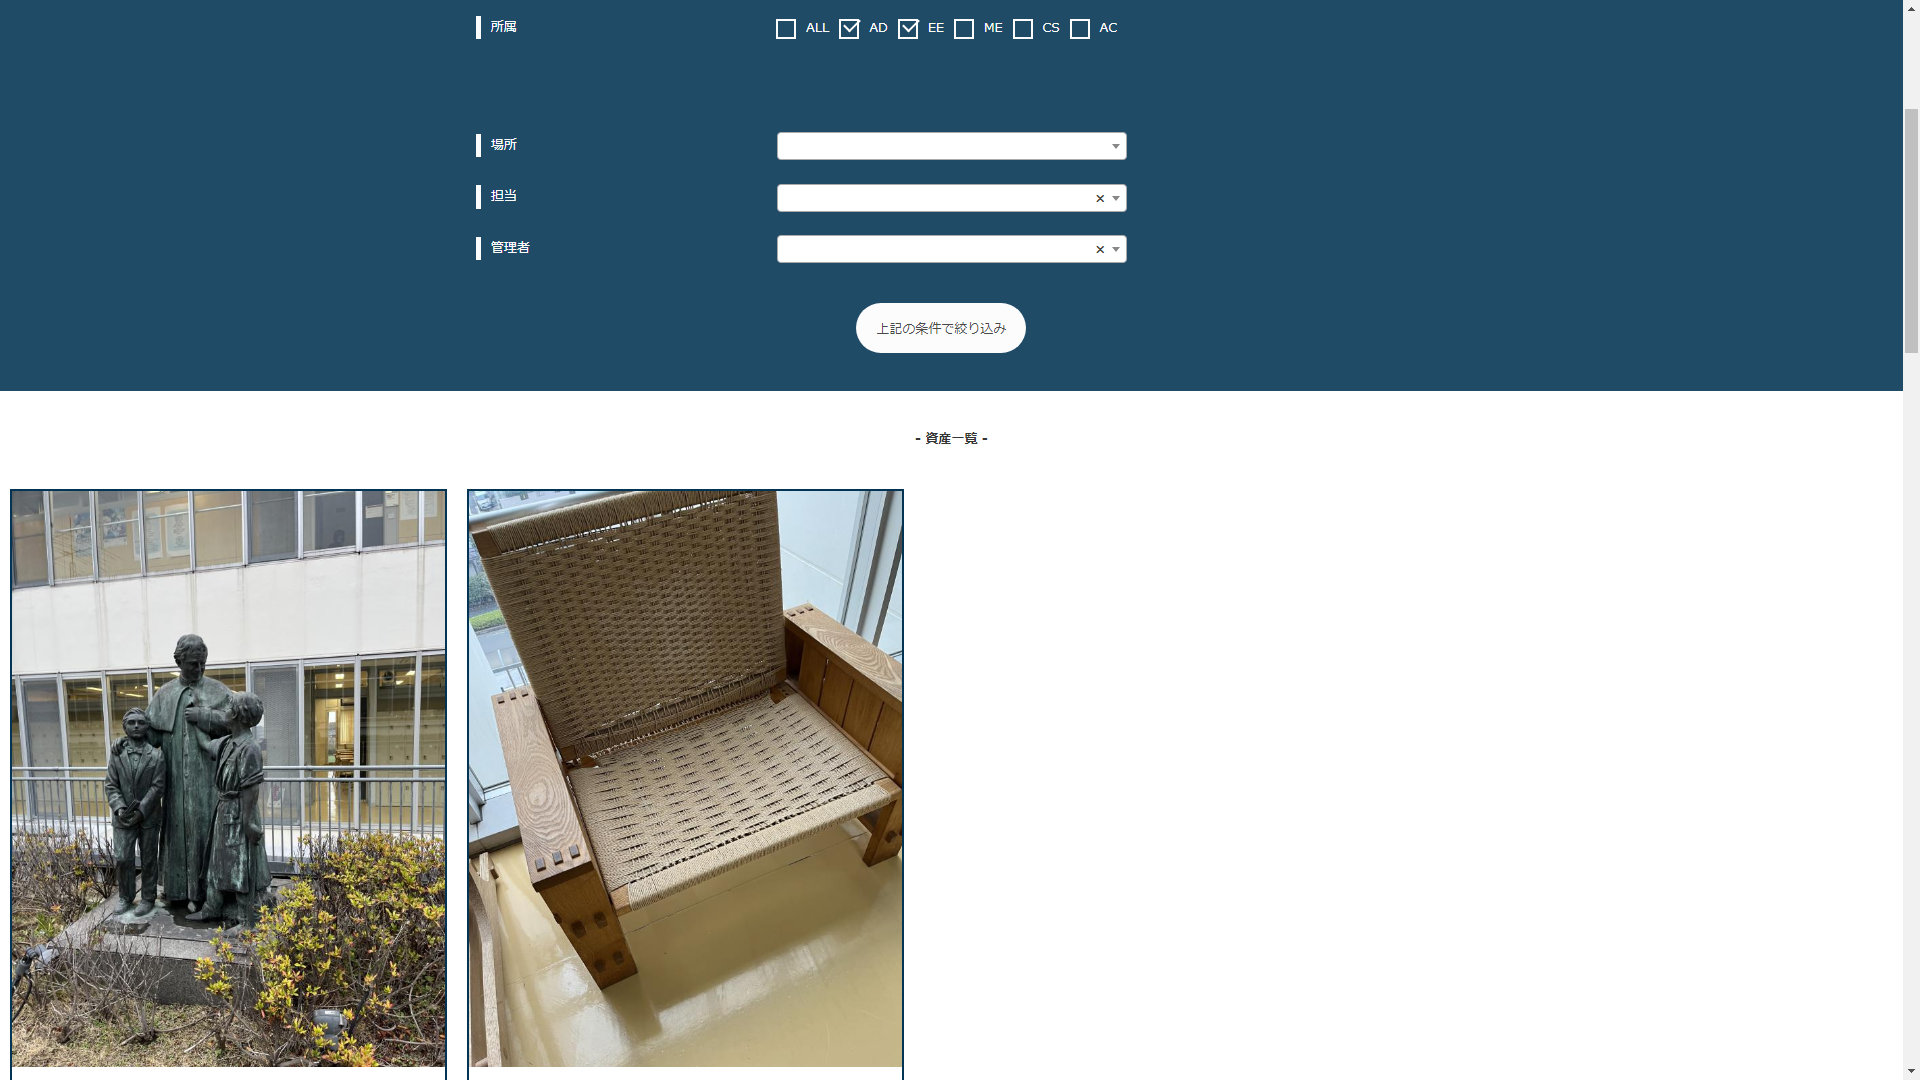
\includegraphics[keepaspectratio, width=0.8\linewidth]{source/search3.png}
  }
  \caption{\label{fig:変化した検索画面}変化した検索画面}
\end{figure}


%%%%%%%%%%
\clearpage
\section{資産の登録}
\label{sec:資産の登録}
資産情報の入力とデータベースへの登録が行えます。登録項目は次の通りです。
\begin{table}[h]
  %\caption{}
  %\label{tb:}
  \centering
  \begin{tabular}{l|l}
    登録可能項目 & 所属・資産名・場所・担当者・管理者・形式・個数・取得年月日・画像(URL)
    \\\hline
    登録必須項目 & 所属・資産名・場所・担当者・管理者・形式
    \\\hline
    登録任意項目 & 個数・取得年月日・画像(URL)
  \end{tabular}
\end{table}
%各項目について入力形式とか詳しく言うかどうか
%Core2Duoは各項目ごとにsubsectionをたてることで「登録手順」としていた 我々は画像で対応したい
%確認画面が表示されるところまで記載
%画像内の説明文をより詳しくするイメージで文章を記述する
\begin{figure}[h]
  \centering
  \fbox{
    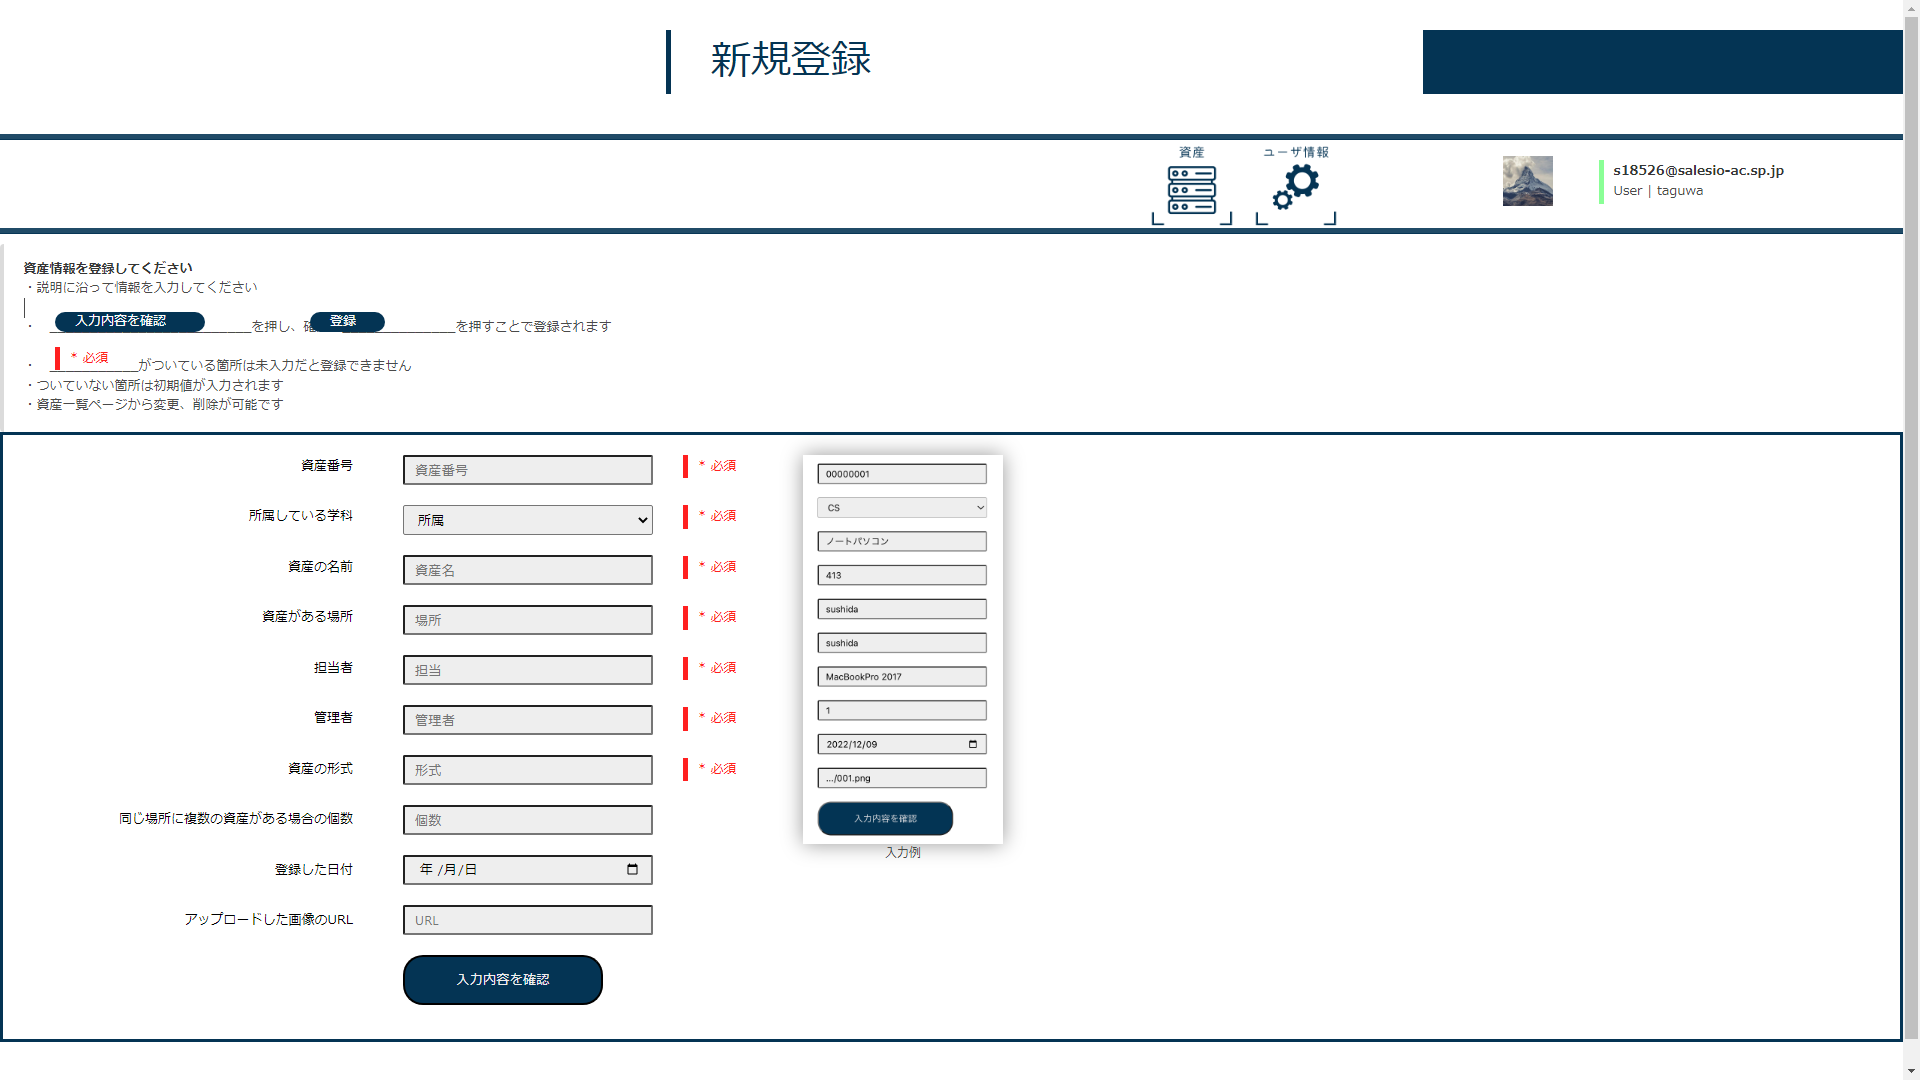
\includegraphics[keepaspectratio, width=0.8\linewidth]{source/submit.png}
  }
  \caption{\label{fig:登録画面}登録画面}
\end{figure}\\
フォームに必要な情報を入力し、\ovalbox{1:入力内容を確認}ボタンを押すと確認画面({\tt image}\ \ref{fig:登録画面の確認表示})が表示されます。\ovalbox{2:登録}ボタンを押すとデータベースに登録されます。\ulinej{登録ボタンを押すまで資産データには反映されません。}\\
{\tt image}\ \ref{fig:入力例}に入力例を示しています。
\begin{figure}[htbp]
  \centering
  \begin{minipage}[h]{0.6\linewidth}
    \centering
    \fbox{
      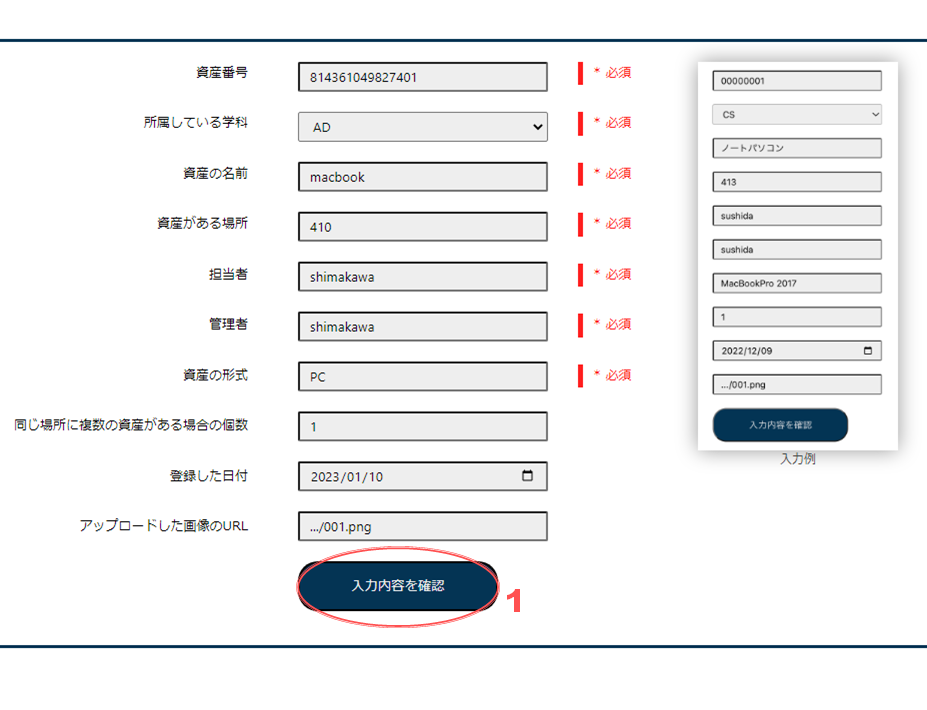
\includegraphics[keepaspectratio, width=\linewidth]{source/submit_example.png}
    }
    \caption{\label{fig:入力例}入力例}
  \end{minipage}
  \hfill
  \begin{minipage}[h]{0.3\linewidth}
    \fbox{
      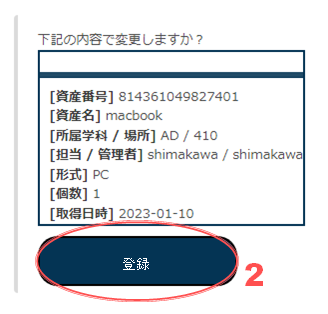
\includegraphics[keepaspectratio, width=\linewidth]{source/submit_verification.png}
    }
    \caption{\label{fig:登録画面の確認表示}登録画面の確認表示}
  \end{minipage}
\end{figure}\\
画面右上の\ovalbox{資産}ボタンからホーム画面へ戻ることができます。


%%%%%%%%%%
\clearpage
\section{資産の編集}
\label{sec:資産の編集}
ホーム画面および検索機能で編集したい資産データを見つけ、ボタンを押すことでこのページにアクセスできます。\\
選択した資産のデータが入力された状態のフォームが表示され、場所・担当者・個数・画像(URL)の内容を編集できるようになっています({\tt image}\ \ref{fig:変更画面})。\ovalbox{1:入力内容を確認}ボタンを押すと確認画面({\tt image}\ \ref{fig:変更画面の確認表示})が表示され、\ovalbox{2:変更}ボタンを押すと登録できます。\\
画面右上の\ovalbox{資産}ボタンからホーム画面へ戻ることができます。
%・登録と同じようにすればいいと思う\\
%・確認画面が表示されるところまで記載\\
%・画像内の説明文をより詳しくするイメージで
\begin{figure}[h]
  \centering
  \fbox{
    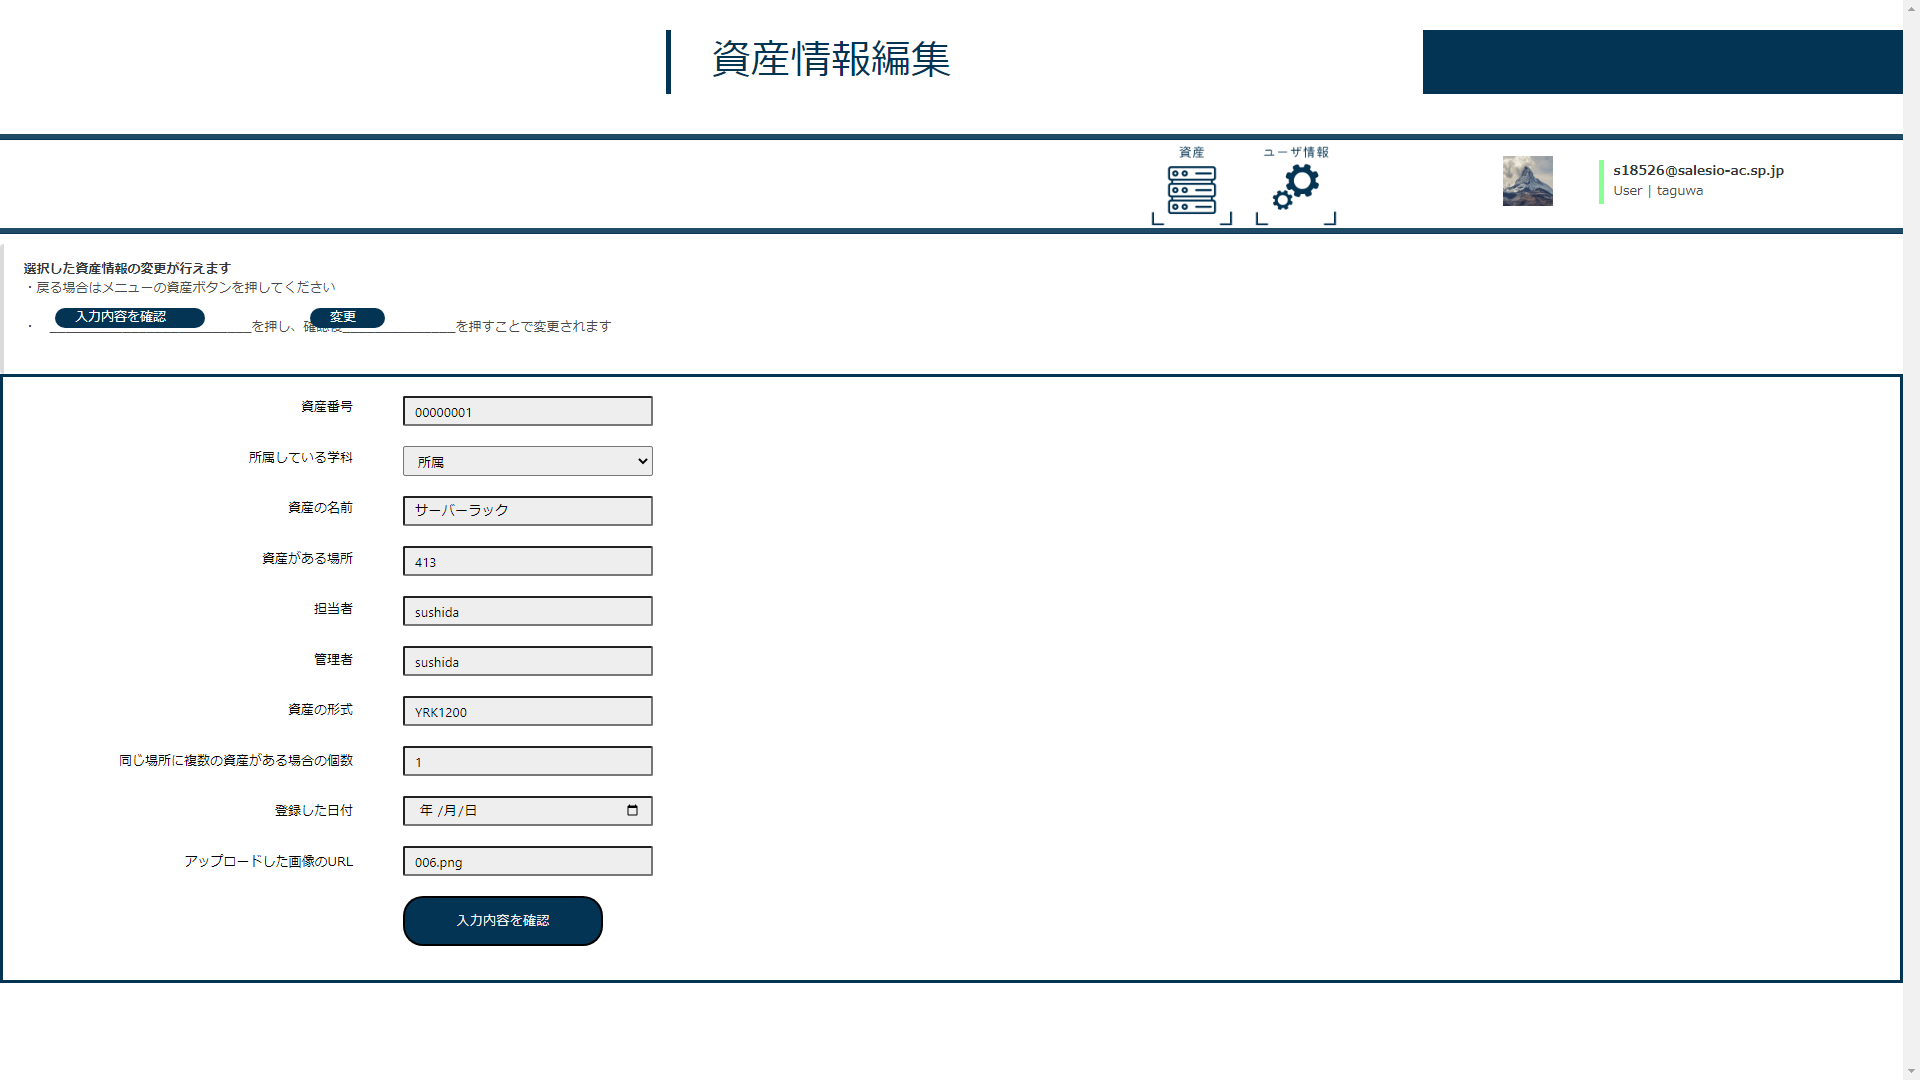
\includegraphics[keepaspectratio, width=0.8\linewidth]{source/change.png}
  }
  \caption{\label{fig:変更画面}変更画面}
\end{figure}
\begin{figure}[h]
  \centering
  \fbox{
    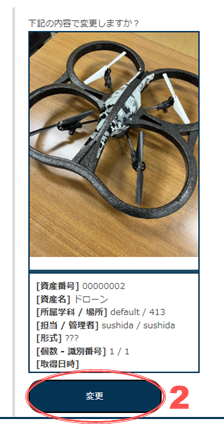
\includegraphics[keepaspectratio, height=0.6\linewidth]{source/change_verification.png}
  }
  \caption{\label{fig:変更画面の確認表示}変更画面の確認表示}
\end{figure}


\begin{comment}
%%%%%%%%%%
\clearpage
\section{資産の削除}
\label{sec:資産の削除}
ホーム画面および検索機能で削除したい資産データを見つけ、削除ボタンを押すことでその資産データを削除できます。\ovalbox{削除}ボタンを押すと確認画面({\tt image}\ \ref{fig:削除の確認表示})が表示され、\ovalbox{{\sf OK}}ボタンを押すと登録できます。\\
画面右上の\ovalbox{資産}ボタンからホーム画面へ戻ることができます。
\begin{figure}[h]
  \centering
  \fbox{
    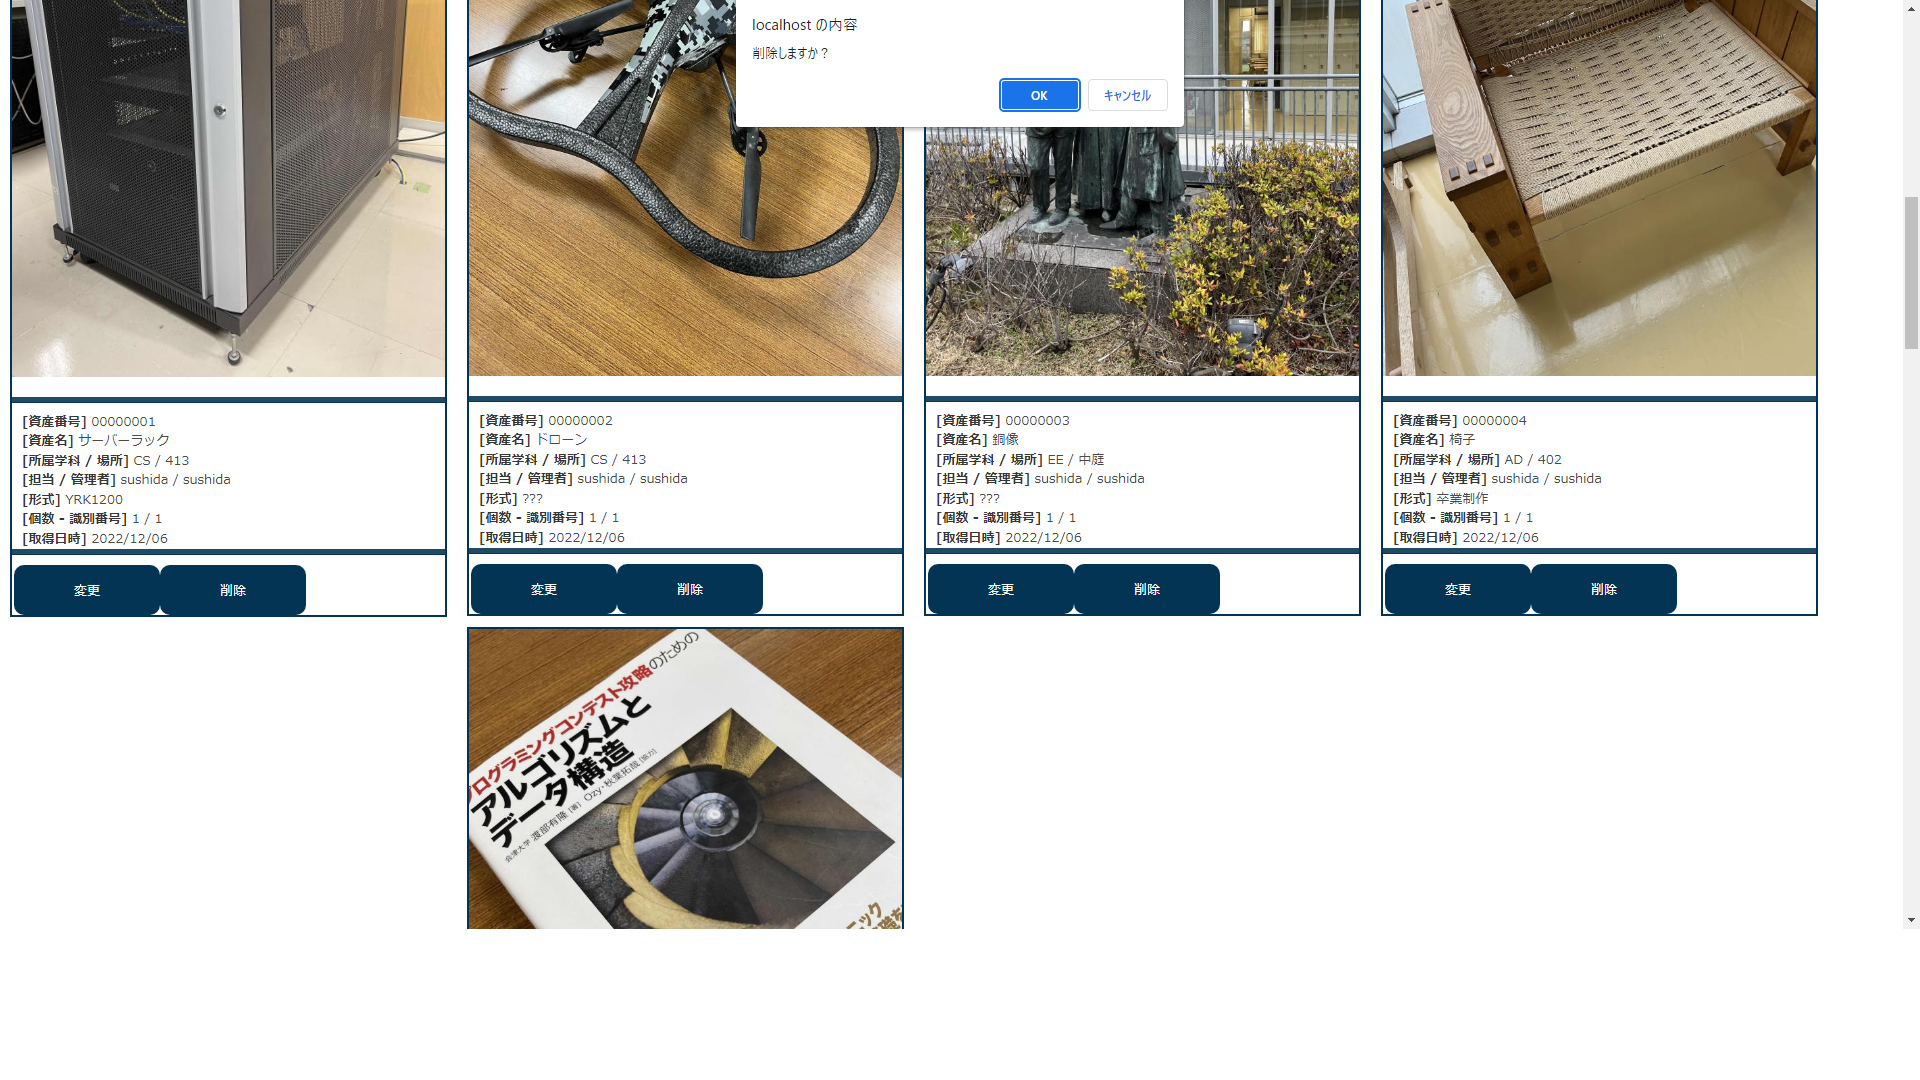
\includegraphics[keepaspectratio, width=0.8\linewidth]{source/delete_verification.png}
  }
  \caption{\label{fig:削除の確認表示}削除の確認表示}
\end{figure}
\end{comment}


%%%%%%%%%%
\clearpage
\section{プロフィールの編集}
\label{sec:プロフィールの編集}
ログインしているユーザ(アカウント)のプロフィールを編集できます。編集できる項目はログインに利用するパスワードのみです。
%・ユーザ情報編集
\begin{figure}[h]
  \centering
  \fbox{
    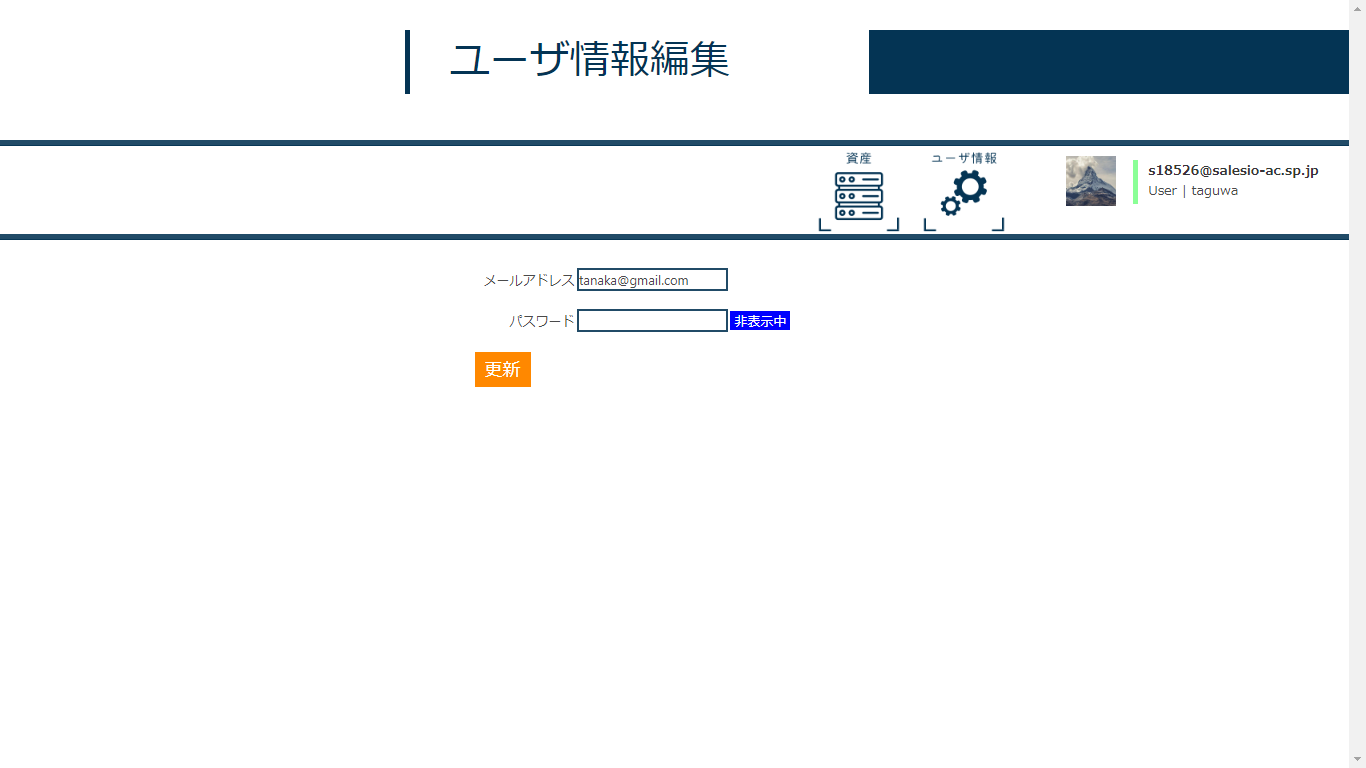
\includegraphics[keepaspectratio, width=0.8\linewidth]{source/user_edit.png}
  }
  \caption{\label{fig:プロフィールの編集画面}プロフィールの編集画面}
\end{figure}
% \section{プロフィールの編集}なので、コメントアウトしました 2023/01/13 11:59 高橋


\begin{comment}
%%%%%%%%%%
\clearpage
\section{ユーザの管理}
\label{sec:ユーザの管理}
本システムに登録されているユーザを一覧し、管理することができます。一覧は学科ごとに分かれて表示され、各データには\ovalbox{1:削除}ボタンが付属しています。\ovalbox{1:削除}ボタンを押すと確認画面({\tt image}\ \ref{fig:ユーザの管理画面の確認表示})が表示され、\ovalbox{2:{\sf OK}}ボタンを押すと登録できます。
\begin{figure}[h]
  \centering
  \begin{minipage}[h]{0.6\linewidth}
    \centering
    \fbox{
      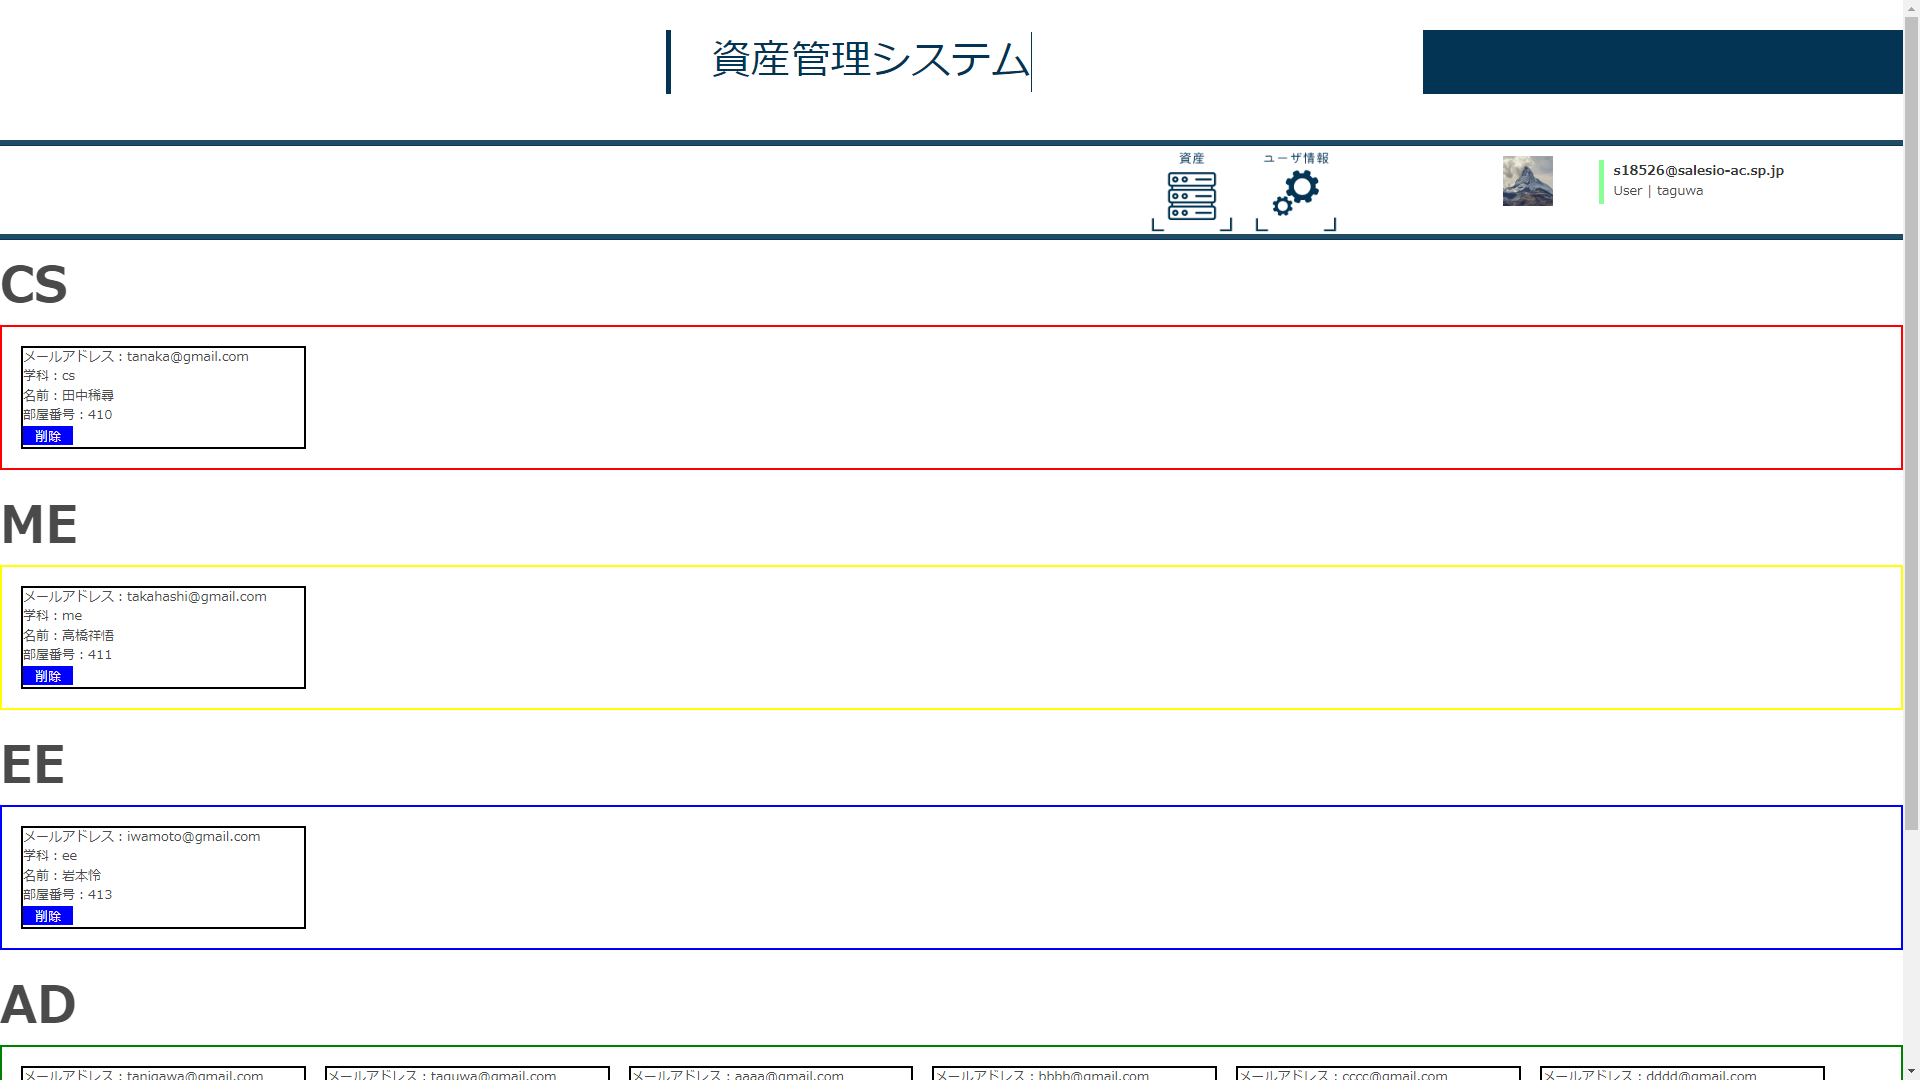
\includegraphics[keepaspectratio, width=\linewidth]{source/user_administration.png}
    }
    \caption{\label{fig:ユーザの管理画面}ユーザの管理画面}
  \end{minipage}
  \hfill
  \begin{minipage}[h]{0.3\linewidth}
    \centering
    \begin{minipage}[h]{\linewidth}
      \fbox{
        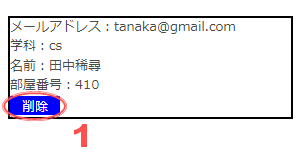
\includegraphics[keepaspectratio, width=\linewidth]{source/numered/user_administration.png}
      }
    \end{minipage}\\
    \bigskip
    \begin{minipage}[h]{\linewidth}
      \fbox{
        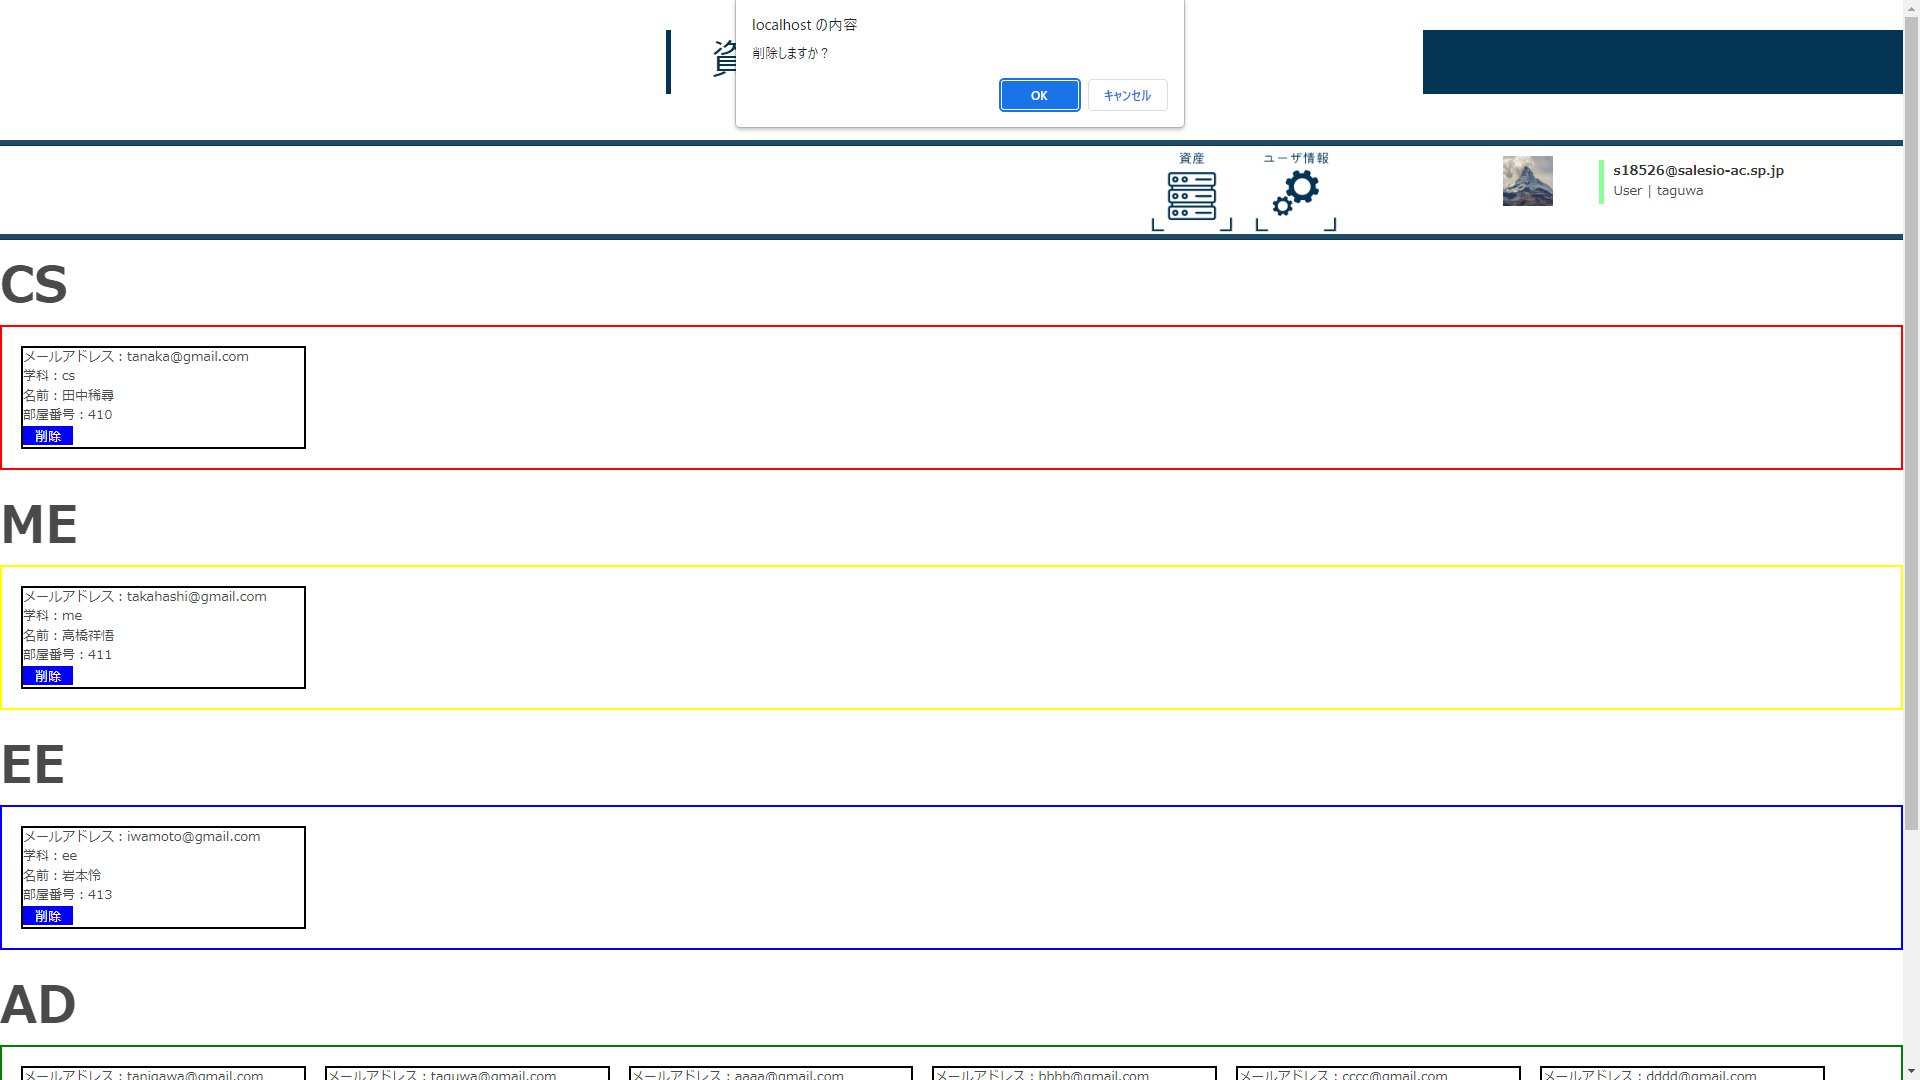
\includegraphics[keepaspectratio, width=\linewidth]{source/user_administration_verification.png}
      }
      \caption{\label{fig:ユーザの管理画面の確認表示}ユーザの管理画面の確認表示}
    \end{minipage}
  \end{minipage}
\end{figure}
\end{comment}


%%%%%%%%%%
%改変履歴
\clearpage

% fancyhdr settings
\thispagestyle{fancy}\thispagestyle{fancy}
\lhead{{\small\bf 一般ユーザ向けマニュアル}}
\chead{}
\rhead{}
\lfoot{}
\cfoot{\thepage}
\rfoot{}
% fansyhdr settings end.

{\Large\bfseries\ 改変履歴}
\begin{table}[htbp]
  %\caption{}
  %\label{tb:}
  \centering
  \begin{tabularx}{\textwidth}{wc{0.2\linewidth}|wl{0.6\linewidth}|wl{0.2\linewidth}}
    日付       & 項目     & 担当者 \\
    \hline \hline
    2023/01/20 & 初版作成 & 高橋   \\
    %\hline
  \end{tabularx}
\end{table}


\end{document}
%%%%%%%%%%%%%%%%%%%
%%%%%%%%%%%%%%%%%%%

%
